\hypertarget{monetaire-expansie}{%
\chapter{Monetaire Expansie}\label{monetaire-expansie}}

\begin{blockquotebox}
    Kredietexpansie kan kapitaal\index{kapitaal} niet vervangen.\footnotemark
    \par\raggedleft--- Ludwig von Mises\index{Ludwig von Mises}
\end{blockquotebox}
\footautocite{166}

\vspace{-1em}
\hypertarget{circulatiekrediet}{%
\section{Circulatiekrediet}\label{circulatiekrediet}}

\lettrine{I}n het vorige hoofdstuk werd uitgelegd hoe goederenkrediet werkt, dat Mises definieert als krediet\index{krediet} dat door banken wordt verstrekt met een perfecte overeenstemming tussen de omvang en de looptijd van de lening\index{lening} van de spaarders aan de bank\index{bank}, en van de bank\index{bank} aan de investeerders. Met andere woorden, goederenkrediet is een krediettransactie waarbij de bank\index{bank} slechts een tussenpersoon is die de afstemming tussen spaarders en investeerders vergemakkelijkt. In elke transactie van goederenkrediet leidt het bedrag van het geïnvesteerde kapitaal\index{kapitaal} tot een uitstel van consumptie\index{consumptie} door de eigenaren van het geïnvesteerde spaargeld voor een gelijk bedrag, wat betekent dat rentetarieven de tijdsvoorkeur\index{tijdsvoorkeur} van de kredietverstrekker weerspiegelen. Dit hoofdstuk gaat over kredietregelingen waarin een investering niet leidt tot een afname van de consumptie\index{consumptie} door de kredietverstrekkers. Volgens wat Mises benoemt als circulatiekrediet, resulteert lenen in de creatie van nieuw geld.

De meest voorkomende manier waarop circulatiekrediet ontstaat, is wanneer financiële instellingen geld uitlenen waarvan ze tegelijkertijd beloven dat het beschikbaar is voor de spaarder. Dit staat in de praktijk ook wel bekend als \textbf{fractioneel bankieren\index{fractioneel bankieren}}. De uitlener, in dit geval de depositohouder van de bank\index{bank}, hoeft de consumptie\index{consumptie} van zijn deposito niet uit te stellen, terwijl het wordt uitgeleend als krediet\index{krediet} aan een ondernemer, zoals het geval is bij goederenkrediet waarbij de spaarder gedurende de hele looptijd van de lening\index{lening} aan de ondernemer afstand doet van zijn deposito. Dit laatste wordt ook wel ``full reserve, maturity matched commodity credit'' genoemd.

Een andere manier waarop een bank\index{bank} circulatiekrediet kan creëren is door de looptijden van haar leningen en deposito\textquotesingle s niet op elkaar af te stemmen. Als de bank\index{bank} alleen krediet\index{krediet} uitleent voor een bedrag gelijk aan haar deposito\textquotesingle s, maar dit ook uitleent met een langere looptijd dan ze heeft geleend, dan creëert ze ook circulatiekrediet. De lening\index{lening} gaat er in feite van uit dat de bank\index{bank} nieuwe depositohouders zal kunnen vinden die bereid zijn geld te storten tegen een lagere rente\index{rente} dan de rente\index{rente} die ze aan de ondernemer biedt. Elke keer wanneer de gouden regel die in Hoofdstuk 14 werd besproken wordt overtreden, komt er dus meer circulatiekrediet in omloop.

Een derde manier waarop circulatiekrediet kan worden gecreëerd is door herhypothecatie van onderpand voor leningen -- het hergebruik van onderpand voor meer dan één lening\index{lening}. Als het onderpand al eerder was verpand voor een lening\index{lening}, dan betekent de tweede lening\index{lening} geen uitstel van consumptie\index{consumptie} voor de kredietverstrekker.

Op al deze drie manieren wordt er krediet\index{krediet} gecreëerd zonder evenredige opoffering van de kant van de kredietverstrekker. Het wordt uitgegeven als \textbf{fiduciaire middelen}: bankbiljetten\index{bankbiljetten} en banksaldi die inwisselbaar zijn voor geld, maar waarvan geen gelijkwaardige geldhoeveelheid beschikbaar is om uitbetaald te worden door de bank\index{bank} wanneer de depositotermijn verloopt.

Geld is, zoals besproken in Hoofdstuk 10, uniek omdat het het enige goed is dat uitsluitend wordt verkregen om weer te worden geruild voor iets anders. Het wordt niet geconsumeerd, zoals consumptiegoederen\index{consumptiegoed}, noch gebruikt bij de productie\index{productie} van andere goederen, zoals kapitaalgoederen\index{kapitaalgoederen}. Aangezien de enige functie van geld is om het om te ruilen en het verder geen fysieke functie heeft voor de eigenaar, kan een vordering erop, of een substituut ervoor, dezelfde rol vervullen terwijl dit niet het geval is voor een substituut of vordering op een ander consumptiegoed\index{consumptiegoed} of kapitaalgoed\index{kapitaalgoederen}. Een coupon voor een biefstuk kan niet worden opgegeten, een coupon voor een machine kan geen goederen produceren, en met een vliegticket kun je niet vliegen. Een vordering op geld kan echter wel de essentiële functie van geld vervullen: het kan worden geruild voor andere goederen. In de woorden van Mises:

\begin{blockquotebox}
    De bijzondere houding van mensen ten aanzien van transacties waarbij circulatiekrediet betrokken is, is te verklaren doordat vorderingen op geld kunnen worden gebruikt voor alle transacties, in plaats van geld zelf. Wie geld nodig heeft, om het uit te lenen, om iets te kopen, om schulden te vereffenen, of om belastingen te betalen, is niet eerst verplicht om de geldvorderingen (biljetten of banktegoeden) om te zetten in geld; de vorderingen zelf kunnen ook direct gebruikt worden als betaalmiddel. Ze zijn dus eigenlijk geldsubstituten; ze vervullen de monetaire functie op dezelfde manier als geld; het is in feite contant geld\index{contant geld} dat direct kan worden uitgegeven, en geen geld dat pas in toekomst beschikbaar wordt.
    \par\vspace{1em}\noindent
    Iemand die duizend broden bezit, zal niet meer dan duizend coupons uitgeven die elke bezitter het recht geven om te allen tijde een brood op te eisen. Met geld ligt dit anders. Omdat niemand geld op zich waardeert, maar het slechts wenst te gebruiken als ruilmiddel voor iets anders, is het zeer wel mogelijk dat er schuldbewijzen voor in de plaats komen. Deze schuldbewijzen kunnen van hand tot hand gaan zonder dat iemand daadwerkelijk probeert het ermee verbonden recht op te eisen.\footnotemark
\end{blockquotebox}
\footautocite{167}

Door hun unieke eigenschappen kunnen fiduciaire middelen, zoals bankbiljetten en bankrekeningen die door de bank\index{bank} zijn uitgegeven, als geld functioneren. Ze kunnen worden gebruikt voor de aankoop van goederen of diensten en als betaling worden geaccepteerd zonder dat ze bij de uitgevende bank\index{bank} ingewisseld moeten worden voor contant geld. Deze fiduciaire middelen dienen als ruilmiddel\index{ruilmiddel}, zonder ze om te moeten zetten in geld. Belangrijk is dat fiduciaire middelen fundamenteel verschillen van bankbiljetten\index{bankbiljetten} die volledig gedekt zijn door contanten, die de bank\index{bank} op verzoek beschikbaar heeft: de uitgifte van fiduciaire middelen vergt geen opoffering van de kant van de uitgever. Wanneer bankbiljetten\index{bankbiljetten} worden uitgegeven met een 100\% dekking, blijft de totale geldhoeveelheid ongewijzigd. Echter, bij de uitgifte van fiduciaire middelen neemt de geldvoorraad toe. Terwijl het delven van goud\index{goud} een kostbare en onzekere activiteit is, waarvan de kosten vaak in de buurt komen van de verwachte opbrengst van het goud\index{goud}, brengt de uitgifte van fiduciaire middelen een uitbreiding van de geldvoorraad met zich mee zonder significante kosten voor de uitgevende bank. Deze toename van de geldhoeveelheid heeft natuurlijk invloed op de marktwaarde van geld, met verstrekkende gevolgen die door de Oostenrijkse School\index{Oostenrijkse School} al meer dan een eeuw zorgvuldig worden geanalyseerd, en die in de volgende secties worden besproken.

\hypertarget{mises-typologie-van-geld}{%
\section{Mises\textquotesingle{} typologie van geld}\label{mises-typologie-van-geld}}

Door de bijzondere aard van geld, als een goed dat niet geconsumeerd wordt, kunnen geldsubstituten en fiduciaire middelen evengoed een monetaire rol spelen als geld zelf, waardoor verwarring kan ontstaan over wat er precies bedoeld wordt met de term ``geld''. Er bestaat een belangrijk onderscheid en het is daarom nuttig om de typologie te volgen die Mises uiteenzette in \emph{The Theory of Money and Credit} en die wordt uitgelegd in \emph{Mises: The Last Knight of Liberalism},\autocite{169} de intellectuele biografie van Mises door Jörg Guido Hülsmann:

\begin{blockquotebox}
    Mises ontwikkelde een uitgebreide typologie van monetaire objecten -- in Mengeriaanse taal kunnen we dit verwoorden als alle dingen die algemeen aanvaard worden als ruilmiddelen. Op het meest fundamentele niveau maakte hij een onderscheid tussen verschillende soorten ``geld in de nauwe zin'' en ``geldsurrogaten of --substituten''. Geld in nauwe zin is een goed op zichzelf, terwijl geldsubstituten daarentegen wettelijke vorderingen zijn op geld in nauwe zin. Ze worden meestal uitgegeven door banken en zijn terugbetaalbaar in echt geld aan de loketten van de bank\index{bank} die ze uitgeeft.
    \par\vspace{1em}\noindent
    Bij het vaststellen van dit fundamentele onderscheid tussen geld en geldvorderingen paste hij cruciale inzichten toe van Böhm-Bawerk\textquotesingle s baanbrekende werk over de economie van rechtspersonen. Hij benadrukte: ``Vorderingen zijn geen goederen; het zijn middelen om beschikking te krijgen over goederen. Dit kenmerkt hun hele aard en economische betekenis.'' Zoals zijn uiteenzetting in latere delen van het boek zou laten zien, is dit onderscheid van groot belang, zowel voor de integratie van de monetaire theorie binnen het kader van Mengers theorie van waarde en prijzen, als voor de analyse van de rol van het bankwezen binnen het monetaire systeem. De kern van zijn theorie over bankieren is een vergelijkende analyse van de economische betekenis van twee zeer verschillende soorten geldsubstituten. Mises merkte op dat geldsubstituten ofwel gedekt kunnen zijn door een overeenkomstige geldhoeveelheid, in welk geval ze ``geldcertificaten'' zijn, of ze kunnen een dergelijke dekking missen, in welk geval ze fiduciaire middelen of ``Umlaufsmittel'' zijn. Mises wijdt het derde en laatste deel van zijn boek aan een analyse van de economische gevolgen van het gebruik van Umlaufsmittel.\footnotemark
\end{blockquotebox}
\footautocite{170}

De term ``geld'' wordt in brede kring gebruikt om te verwijzen naar zowel geld als geldsubstituten. Mises verduidelijkt het onderscheid op een manier die de Oostenrijkse analyse van de conjunctuurcyclus\index{conjunctuurcyclus} helpt verklaren. Geld, in de nauwere zin, kan drie vormen aannemen:

\vspace{1em}\noindent\textbf{Goederengeld}: Een algemeen ruilmiddel\index{ruilmiddel} dat ook een economisch\index{economisch} goed is en kan worden geruild met goederen van hetzelfde type. Het wordt verkocht op een open markt met veel producenten en consumenten. Historische voorbeelden zijn voornamelijk edelmetalen, maar recentelijk kan bitcoin\index{bitcoin} worden toegevoegd als een nieuwe vorm van een niet-metaal digitaal\index{digitaal} goed.

\vspace{1em}\noindent\textbf{Kredietgeld}: Een toekomstige financiële vordering op een rechtspersoon die wordt gebruikt als ruilmiddel\index{ruilmiddel}. Wat kredietgeld onderscheidt van krediet\index{krediet}, is dat de ontvanger het accepteert met de bedoeling het door te geven aan een andere ontvanger, niet omdat hij de financiële vordering wil innen.

\vspace{1em}\noindent\textbf{Fiatgeld}: Een ruilmiddel\index{ruilmiddel} dat geaccepteerd wordt op basis van een wettelijk besluit van een autoriteit. ``De beslissende factor is de stempel van de overheid\index{overheid}. Het is niet het materiaal dat de stempel draagt dat het geld vormt, maar de stempel zelf.''\autocite{171} Fiatgeld kan de vorm aannemen van papiergeld, bankdeposito\textquotesingle s of munten\index{munten}.

\vspace{1em}\noindent Hoewel geldsubstituten vaak met echt geld worden verward, zijn ze in feite verschillend.

\vspace{1em}\noindent\textbf{Geldsubstituten}: Fysieke of financiële instrumenten die wettige vorderingen zijn van geld in nauwe zin. Ze kunnen op verzoek worden ingewisseld voor geld en worden gebruikt als ruilmiddel\index{ruilmiddel} bij transacties. Geldsubstituten zijn er in twee vormen:

\vspace{1em}\noindent\textbf{Geldcertificaten}: Een financieel instrument of papier dat op verzoek volledig inwisselbaar is voor geld (de waarde wordt 100\% gedekt door de uitgevende instantie.) Voorbeelden zijn een dollarbiljet dat in goud\index{goud} kan worden ingewisseld onder een strikte goudstandaard\index{goudstandaard}, of een bankrekening gebaseerd op dollars met goud\index{goud} als onderpand. Op het gebied van bitcoin\index{bitcoin} kunnen we bitcoin\index{bitcoin} op het lightningnetwerk beschouwen als een uniek type geldcertificaat, omdat de werking ervan volledig in handen is van de houder van het geld en de terugbetaling niet afhankelijk is van derden. Verhandelbare eigendomsbewijzen voor bitcoin\index{bitcoin} die door een derde partij in bewaring worden gehouden zouden ook geldcertificaten zijn. En hoewel deze een tegenpartij zouden hebben die het uitgeeft, zouden ze nog steeds relatief goedkoop en gemakkelijk inwisselbaar zijn voor bitcoin\index{bitcoin}, omdat toegang tot het netwerk niet gemakkelijk te censureren is.

\vspace{1em}\noindent\textbf{Fiduciaire middelen}: Geldsubstituten die niet gedekt worden door een onderpand. Wanneer een financiële instelling geldsubstituten uitgeeft, maar niet het geld heeft om alle substituten terug te betalen, is er sprake van fiduciaire middelen. Dit is een sleutelterm in Mises\textquotesingle{} uitleg van de conjunctuurcyclus\index{conjunctuurcyclus}, want het is precies de creatie van deze middelen die de conjunctuurcyclus\index{conjunctuurcyclus} in gang zet. In het digitale domein zou dit het equivalent zijn van krediet\index{krediet}, uitgedrukt in bitcoin\index{bitcoin}, maar dat wordt uitgegeven zonder het equivalent aan bitcoin\index{bitcoin} als dekking.

\begin{figure}[H]
\centering
    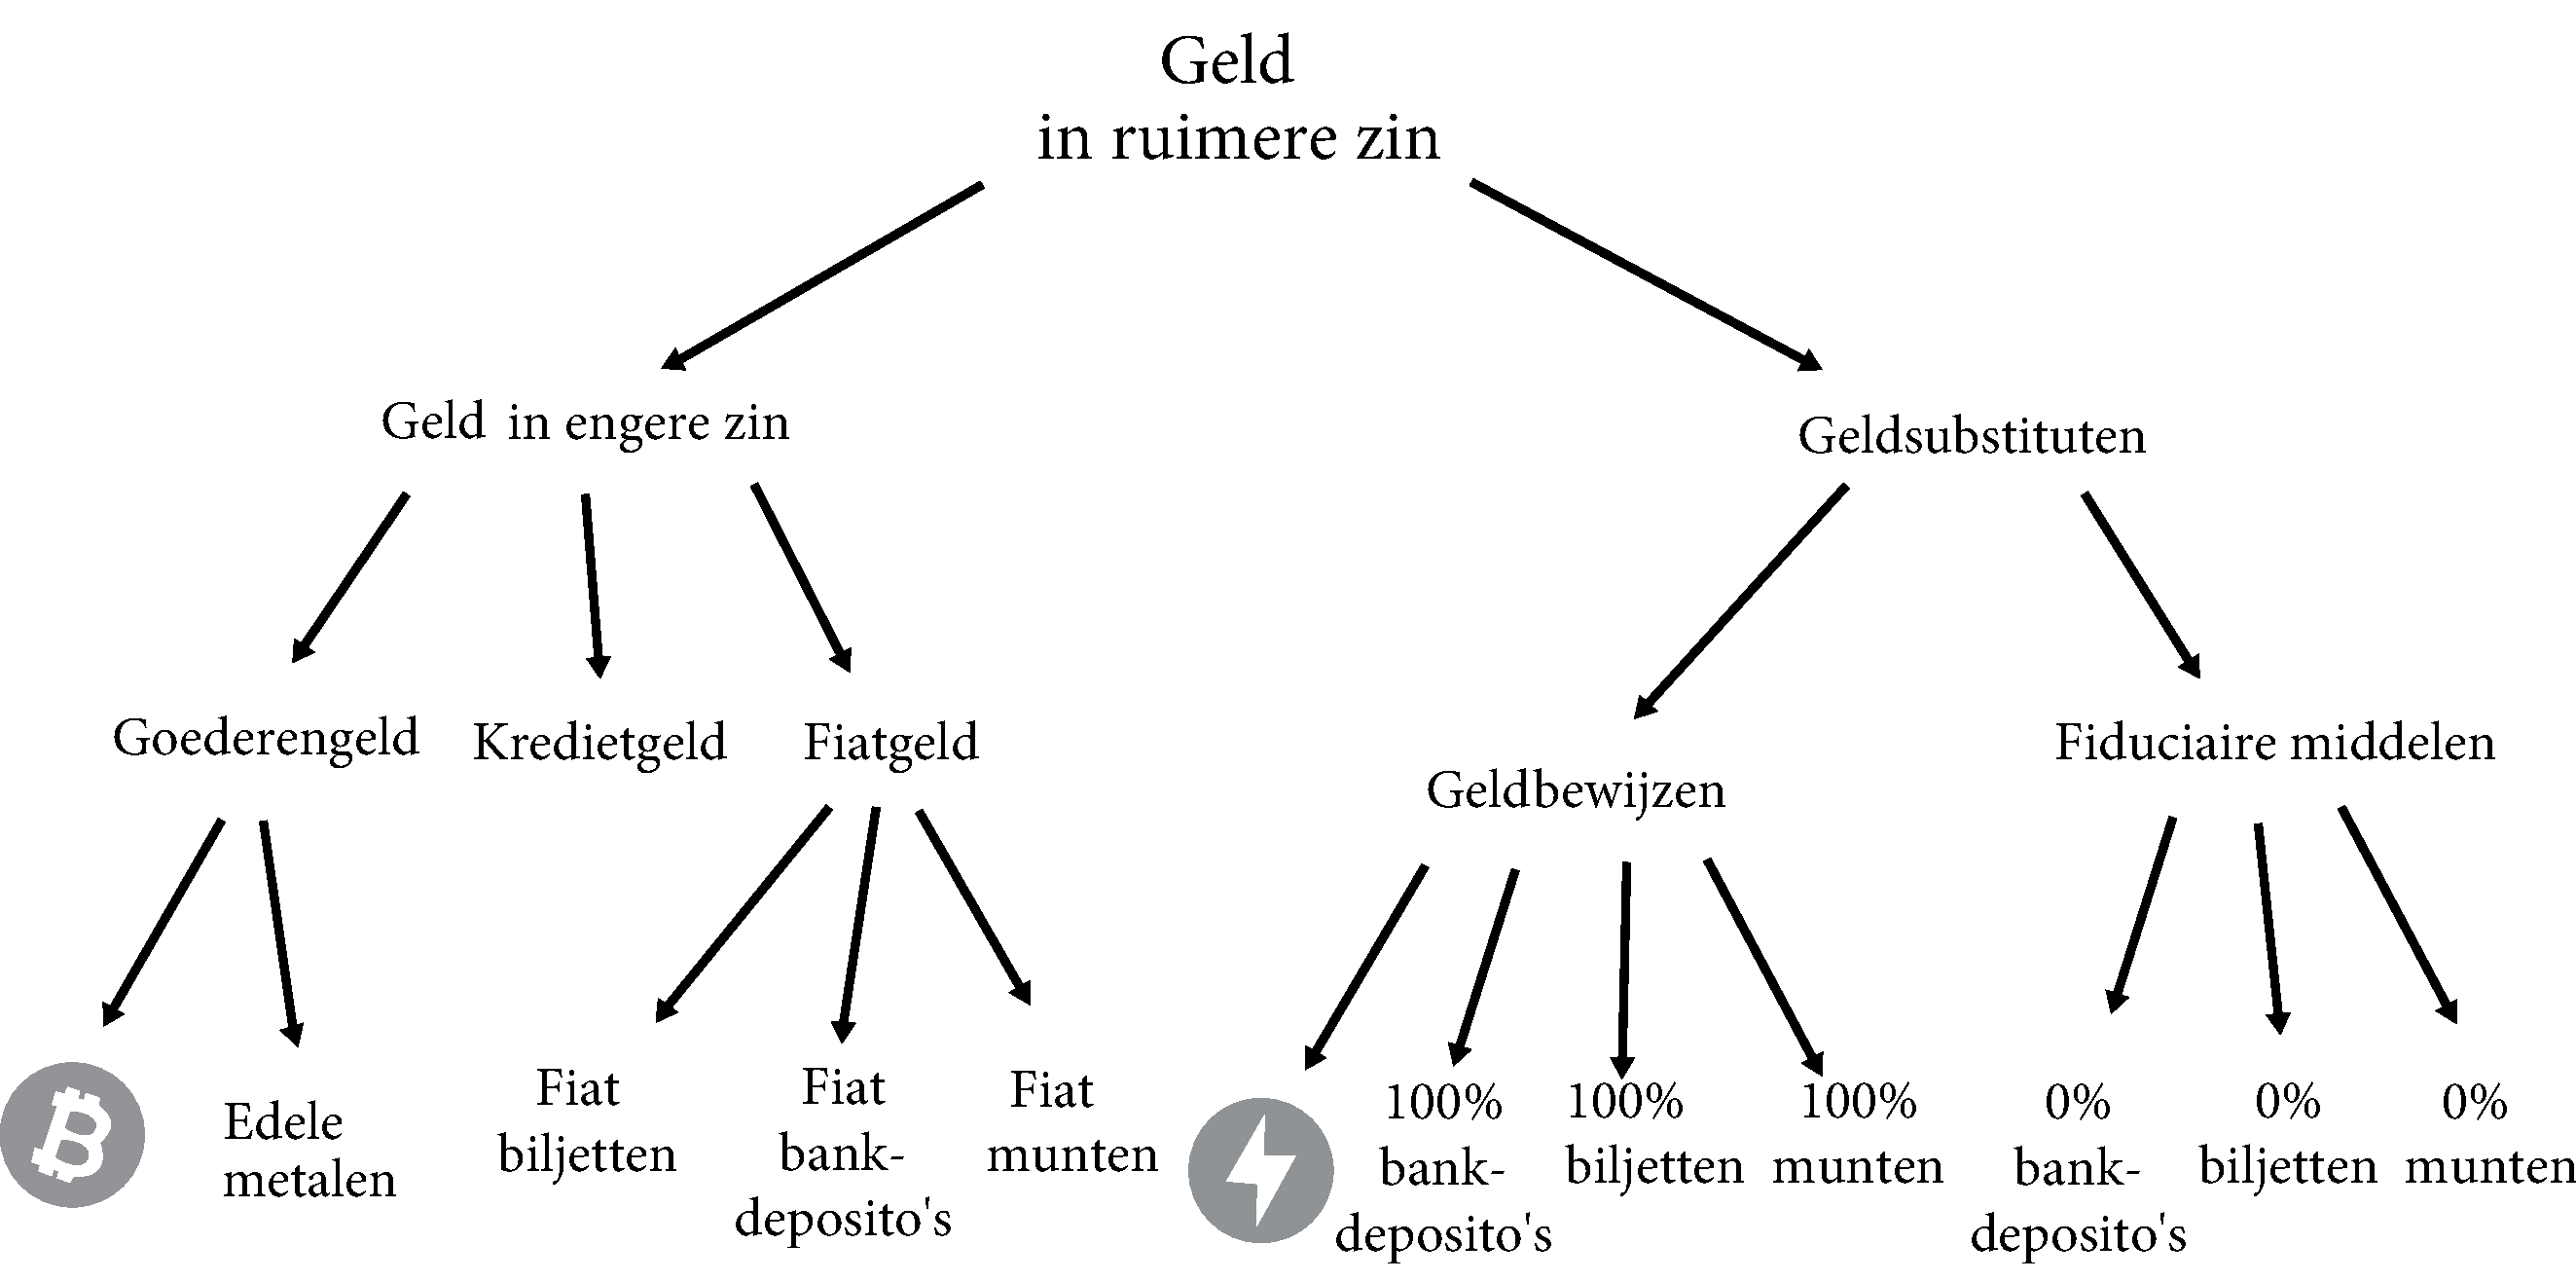
\includegraphics[width=\textwidth]{figures/fig31.pdf}
    \caption[Typologie van geld]{Typologie van geld\footnotemark}
    \label{fig31}
\end{figure}
\footautocite{172}

Volgens de typologie van Mises staat de functie van geld los van zijn fysieke verschijning. Bankdeposito\textquotesingle s nemen de vorm van geldcertificaten aan wanneer ze volledig terugbetaalbaar zijn voor geld, van fiduciaire middelen wanneer ze uitgegeven worden door banken zonder dat er een onderpand tegenover staat, of van fiatgeld\index{fiatgeld} wanneer ze worden door de overheid\index{overheid} worden opgelegd. Volgens hetzelfde principe kan papiergeld een volledig gedekt geldcertificaat zijn en dus inwisselbaar zijn voor het onderliggende goederengeld tegen de nominale waarde, zoals dit was onder de goudstandaard\index{goudstandaard}. Als het echter uitgegeven wordt door een bank\index{bank} en niet terugbetaalbaar is voor geld, dan is het fiduciair geld; en het is fiatgeld\index{fiatgeld} als het gedrukt wordt door een overheid\index{overheid} zonder dat terugbetaling mogelijk is. Fysieke munten\index{munten} kunnen worden gemaakt als goederengeld, zoals gouden en zilveren munten\index{munten}; als fiduciaire middelen wanneer ze worden uitgegeven door een bank\index{bank}; als een geldcertificaat als het inwisselbaar is voor geld; of als fiatgeld\index{fiatgeld} als het wordt geslagen uit een basismetaal en de waarde onafhankelijk van het metaalgehalte wordt bepaald door een autoriteit. Door afstand te nemen van de fysieke verschijningsvormen van het geld en het verschil uit te leggen tussen fiduciaire middelen en geldcertificaten, kon Mises een verklaring geven voor het ontstaan van conjunctuurcycli op basis van menselijk handelen\index{menselijk handelen}.

Bij geldcertificaten is een gelijk bedrag aan geld in de nauwe zin opeisbaar door de houder bij de uitgevende instelling geplaatst; de uitgifte ervan veroorzaakt geen toename van de monetaire middelen in omloop. Wanneer het geldcertificaat op een bepaald moment voor een betaling wordt gebruikt, blijft het geld als dekking in een bankkluis liggen, maar verandert in feite van eigenaar. Dat geld kan geen monetaire transacties afwikkelen, terwijl de geldcertificaten in omloop zijn. Zodra het geldcertificaat is ingewisseld voor het geld in engere zin, kan het worden uitgegeven, maar het bewijs niet meer. Geldcertificaten vergroten de geldhoeveelheid in ruimere zin niet. De introductie van geldsubstituten in de vorm van fiduciaire middelen resulteert daarentegen wel in een toename van de totale geldhoeveelheid en geldsubstituten die in omloop zijn.

In het verleden verrijkten koningen zichzelf ten koste van hun volk door munten\index{munten} van hun onderdanen te verzamelen, het edelmetaalgehalte te verlagen door er onedele metalen in te vermengen, en vervolgens de munten\index{munten} opnieuw te slaan. Door onedele metalen aan de mix toe te voegen, kon de koning meer munten\index{munten} maken dan de hoeveelheid edelmetaal die hij had. Hierdoor kreeg hij zelf meer koopkracht ten koste van de eigenaars van de oorspronkelijke munt. Na verloop van tijd zou de prijs\index{prijs} van goederen stijgen als weerspiegeling van de daling van het edelmetaalgehalte. Een deel van ieders werkelijke rijkdom werd dus overgedragen aan de koning.

Hoewel moderne gecentraliseerde overheden hun fysieke munten\index{munten} niet langer ontwaarden, bereiken ze toch iets vergelijkbaars door wetgeving, dreiging met geweld en door hun monopoliemacht te gebruiken om mensen te dwingen om geldcertificaten die niet langer in geld kunnen worden terugbetaald te accepteren alsof het geld is. Nu ze niet meer inwisselbaar zijn, worden de geldcertificaten fiduciaire middelen, waardoor de totale geldhoeveelheid toeneemt. Op dezelfde manier waarop koningen profiteerden van het mengen van onedele metalen met edele metalen, profiteren moderne overheden van het mengen van fiduciaire middelen met geld. De gevolgen gaan in beide gevallen verder dan alleen het verrijken van de overheid\index{overheid} ten koste van de samenleving. Het introduceren van een goedkope aanvulling op het geld verbetert de functie ervan niet; het brengt het in gevaar. Geld onderscheidt zich van andere goederen doordat de absolute hoeveelheid niet van belang is voor de eigenaar, alleen de koopkracht doet er toe. Het verhogen van de geldhoeveelheid vergroot het vermogen niet, noch maakt het het geld effectiever; in plaats daarvan devalueert het de rijkdom van de huidige eigenaars en draagt het over aan de ontvangers van het nieuw gecreëerde geld. Het zal de prijzen van goederen veranderen waardoor uiteindelijk economische miscalculaties zullen ontstaan.

\hypertarget{conjunctuurcycli}{%
\section{Conjunctuurcycli}\label{conjunctuurcycli}}

De gangbare economische stromingen zijn uiterst voorzichtig bij het beantwoorden van de vraag wat de oorzaak is van conjunctuurcycli, en daar is een goede reden voor. Aangezien de moderne economische wetenschap grotendeels door centrale banken wordt gefinancierd om informatie voor beleidsvorming te leveren, is het erg onwaarschijnlijk dat iemand wiens conclusies niet vleiend zijn voor centrale banken een succesvolle carrière kan verwachten.\autocite{173} Mainstream economisch\index{economisch} onderzoek heeft zich voornamelijk gericht op discussies over hoe recessies kunnen worden voorkomen en gaf daarbij zeer weinig aandacht voor wat recessies eigenlijk veroorzaakt. Het is kinderachtig om te proberen een probleem op te lossen zonder de oorzaken ervan te begrijpen, maar met fiatgeld\index{fiatgeld} kunnen centrale banken proberen hun eigen realiteit te creëren. Dit doen ze door onderzoek te financieren dat gericht is op het vinden van oplossingen en door wetenschappers die kritisch staan tegenover centrale banken te marginaliseren. Deze benadering werd het best geïllustreerd in Krugmans inleiding op een recente herdruk van Keynes\textquotesingle{} \emph{General Theory}, waarin Krugman het onvermogen van Keynes om een verklaring te bieden voor de oorzaken van de conjunctuurcyclus\index{conjunctuurcyclus} prijst:

\begin{blockquotebox}
    In plaats van zich te verliezen in een poging om de dynamiek van de conjunctuurcyclus\index{conjunctuurcyclus} te verklaren -- een onderwerp dat tot op de dag van vandaag omstreden blijft -- richtte Keynes zich op een vraag die beantwoord kon worden. En die ... het hardst een antwoord nodig had: hoe kunnen we dan meer werkgelegenheid creëren als de algemene vraag laag is -- ongeacht de oorzaak?\footnotemark
\end{blockquotebox}
\footautocite{174}

Om succesvol te zijn in de moderne academische wereld is het vooral vereist om loyaal te zijn aan de centrale banken, in plaats van de coherentie of de waarde van je ideeën. Als gevolg daarvan wordt de conjunctuurcyclus\index{conjunctuurcyclus} nog steeds voorgesteld als een normaal, onvermijdelijk onderdeel van de werking van een moderne kapitalistische economie. Het zou net zo onvermijdelijk zijn als de overgang van dag naar nacht.

In schril contrast hiermee bieden de Oostenrijkse economen, met hun realistische raamwerk voor het begrijpen van de wereld dat is gebaseerd op causale verbanden, een coherente verklaring voor waarom conjunctuurcycli plaatsvinden en hoe ze kunnen worden voorkomen. Doordat ze de standpunten van de centrale bankiers niet hoeven te volgen om financiering veilig te stellen, zijn de Oostenrijkers in staat om meer te bieden dan de dubieuze Keynesiaanse aanbevelingen om uit de depressie\index{depressie} te komen: ze kunnen zelfs uitleggen hoe een depressie\index{depressie} voorkomen kan worden.

De Oostenrijkse theorie van de conjunctuurcyclus\index{conjunctuurcyclus} is gebaseerd op en een natuurlijke expansie van de Oostenrijkse theorie van het geld en het eerder genoemde verschil tussen fiduciaire middelen en geld. De hoofdgedachte van de theorie is het eenvoudige idee dat economische middelen niet tevoorschijn kunnen worden getoverd door er ongedekte vorderingen voor te creëren. Dat klinkt misschien als iets logisch dat je met gezond verstand zou beamen, maar voor de meeste moderne economen is het een radicaal concept. Pogingen van overheden en banken om ongedekte vorderingen op economische middelen als gelijkwaardig aan de middelen of aan gedekte vorderingen erop te laten gelden, resulteren in een toename van de geldhoeveelheid, die zich manifesteert als een toegenomen hoeveelheid financieel kapitaal\index{kapitaal} dat beschikbaar komt voor ondernemers. Het toegenomen financiële kapitaal\index{kapitaal} zorgt ervoor dat ondernemers investeringen doen waarvoor ze over onvoldoende middelen beschikken, iets wat pas duidelijk wordt nadat ze hun financiële kapitaal\index{kapitaal} beginnen uit te geven. Dit veroorzaakt een onverwachte prijsstijging van hun inputgoederen, waardoor ze de projecten uiteindelijk niet zullen kunnen afmaken.

In een economie waarin alleen goederenkrediet circuleert, wordt het rentetarief bepaald door de interactie van individuele voorkeuren voor lenen en uitlenen tegen verschillende rentetarieven. De voorkeuren van deze individuen om geld aan te houden, te lenen of uit te lenen worden bepaald door de hoeveelheden geld waarover ze beschikken, en door hun economische omstandigheden en wensen. In een wereld met alleen goederenkrediet moeten alle leningen afkomstig zijn van een spaarder die besluit af te zien van consumptie\index{consumptie} ten gunste van een positief rendement op het uitgeleende geld.

De spaar- en consumptiebeslissingen met betrekking tot financieel kapitaal\index{kapitaal} komen rechtstreeks overeen met de consumptie\index{consumptie}- en spaarbeslissingen voor fysiek kapitaal\index{kapitaal}. De mensen die afzien van de consumptie\index{consumptie} van financieel kapitaal\index{kapitaal}, doen dit door de consumptie\index{consumptie} van economische goederen en diensten die ze ermee hadden kunnen kopen, uit te stellen. Deze niet-geconsumeerde middelen kunnen in plaats daarvan worden ingezet voor het productieproces\index{productieproces} en dus worden geïnvesteerd in productieve ondernemingen.

Een voor de hand liggend voorbeeld is dat de consument die besluit om zijn maïs niet op te eten, het mogelijk maakt om de maïs te gebruiken als zaad voor een volgende oogst. Een uitgebreider voorbeeld uit een complexe economie gaat als volgt: een consument besluit af te zien van een bezoek aan een strandresort. Dit vermindert de vraag naar personeel in het resort en verkleint de kans dat het resort een nieuw stuk grond koopt om uit te breiden. Hij stort het geld dat hij aan de reis zou hebben uitgegeven op een spaarrekening bij zijn bank\index{bank}, waardoor de bank\index{bank} dit geld nu kan uitlenen aan een autofabrikant, die zich hierdoor een extra werknemer kan veroorloven die niet door het strandresort is ingehuurd. Hij kan misschien zelfs het stuk grond kopen dat het resort eerst in gebruik had willen nemen. Door zijn vakantie op te geven en ervoor te kiezen zijn geld aan ondernemers uit te lenen, heeft de spaarder middelen vrijgemaakt die zouden zijn gebruikt voor consumptie\index{consumptie} in de vorm van een vakantie. Deze middelen kunnen nu ingezet worden voor de productie\index{productie} van auto\textquotesingle s.

Schaarste is het fundamentele uitgangspunt van economie; geld en financiële instellingen zijn hulpmiddelen die we gebruiken om te sparen, onze productiviteit en efficiëntie te verhogen en om schaarste\index{schaarste} te bestrijden, maar ze kunnen de schaarste\index{schaarste} van middelen niet opheffen. Er is altijd een beperkte hoeveelheid werknemers, kantoorruimte, apparatuur, computers, land en grondstoffen, en het verhandelen ervan met geld is de manier waarop we de middelen inzetten. Zolang een economie werkt op basis van goederenkrediet, worden financiële middelen gekoppeld aan echte middelen waardoor consumptiebeslissingen daadwerkelijk individuele voorkeuren weerspiegelen met betrekking tot echte middelen. Deze voorkeuren worden uitgedrukt in de prijzen.

Dit proces wordt verstoord door de introductie van fiduciaire middelen, die circuleren als geld maar niet door geld worden gedekt. Wanneer een financiële instelling een lening\index{lening} verstrekt zonder dat daar geld tegenover staat, geeft ze krediet\index{krediet} uit zonder een overeenkomstig uitstel van consumptie\index{consumptie} door een consument. De bank\index{bank} heeft een vorderingsbewijs uitgegeven aan de boer om zaaigoed te kopen dat al is opgegeten. Het totale bedrag aan leningen dat is uitgegeven om zaaigoed te kopen is hoger dan de huidige marktwaarde van alle zaaigoed dat over is gebleven van de oogst van vorig jaar. De bank\index{bank} heeft de autofabrikant het geld gegeven om grond te kopen en arbeiders in te huren, terwijl de vakantieganger ook zijn geld in het resort heeft uitgegeven, waardoor het resort dezelfde arbeiders kon inhuren en hetzelfde land kon kopen.

Wanneer de fiduciaire middelen worden gecreëerd als een lening\index{lening} aan ondernemers, is het misschien voor niemand duidelijk (behalve voor Misesiaanse economen) dat deze lening\index{lening} meer vorderingen heeft gecreëerd dan er middelen zijn. Tegen de huidige maïsprijzen is de hoeveelheid maïs die boeren van plan zijn te kopen groter dan de hoeveelheid zaaigoed dat beschikbaar is op de markt. Maar zodra het plantseizoen is aangebroken en de boeren het zaaigoed gaan kopen, bieden ze de prijs\index{prijs} snel op. Degenen die het zaaigoed vroeg kopen, krijgen misschien de hele hoeveelheid die ze van plan waren te kopen, maar de meerderheid krijgt een kleinere hoeveelheid. Deze miscalculatie zal een dure fout zijn voor de boeren, die te veel geïnvesteerd hebben in grond, arbeid en kapitaal\index{kapitaal} in verhouding tot de hoeveelheid zaad die ze beschikbaar hebben.

Het vakantieoord en de autofabriek verwachten allebei dat hun geldvoorraad en fiduciaire middelen voldoende zullen zijn om het stuk grond en de arbeiders die ze nodig hebben te kunnen betalen. Zodra ze de arbeiders echter daadwerkelijk gaan inhuren en het land gaan kopen, zullen de toegenomen fiduciaire middelen leiden tot een daling van de waarde van het geld ten opzichte van de inputgoederen, waardoor de prijzen zullen stijgen. Als de eigenaar van het stuk grond biedingen ontvangt van zowel het vakantieoord als de autofabriek, begint er een biedingsstrijd tussen de twee en er zal een hogere prijs\index{prijs} tot stand komen. Omdat werknemers kansen vinden bij beide bedrijven, stijgen ook hun lonen. Omdat fiduciaire middelen door het verlagen van de rentetarieven de banken en ondernemers een vertekend beeld geven van de middelen die werkelijk voor hen beschikbaar zijn, beginnen veel zakelijke kansen winstgevend te lijken in de berekeningen van ondernemers, terwijl de werkelijk beschikbare middelen niet voldoende zijn om ze tot een goed einde te brengen.

Nu de kosten van grond, arbeid en kapitaalgoederen\index{kapitaalgoederen} de pan uit rijzen, zijn de plannen van de twee ondernemers in duigen gevallen. Ze hadden alle economische calculaties uitgevoerd op basis van prijzen die golden voordat de fiduciaire middelen in omloop werden gebracht. Door de stijgende prijzen van de inputgoederen, worden hun eerdere berekeningen helaas nutteloos. Hun winstgevendheid vermindert of verdwijnt, en ze zouden allebei failliet\index{faillissement} kunnen gaan waardoor hun werk en investeringen verloren gaan.

Een zakelijke kans waarvan wordt verwacht dat het een rendement van 4\% zal opleveren, zal geen kapitaal\index{kapitaal} aantrekken van kredietverstrekkers wanneer de gangbare marktrente 6\% is. Maar wel als de introductie van fiduciaire middelen ertoe leidt dat de rente\index{rente} daalt tot 3\%. Hetzelfde bedrijf\index{bedrijf}, met dezelfde kapitaalvoorraad, in dezelfde markt, verandert hierdoor van verlieslatend naar winstgevend. Dit kan alleen maar door de introductie van fiduciaire middelen die tegen verwaarloosbare kosten geproduceerd kunnen worden. De absurditeit van de situatie zou duidelijk moeten zijn: geld is een goed dat op zichzelf geen waarde heeft, en het wordt gespaard om weer verruild te worden. De hoeveelheid doet er niet toe, alleen de koopkracht. Het maken van meer geldeenheden kan niets veranderen aan de economische realiteit van bedrijven waarvan de input en output kapitaalgoederen\index{kapitaalgoederen} en consumptiegoederen\index{consumptiegoed} zijn. Als ze plotseling winstgevend blijken te zijn, kan dat alleen te danken zijn aan de gebrekkige aard van het gebruikte geld.

De financiële problemen van deze verlieslatende bedrijven komen aan het licht wanneer ze de prijzen van hun inputgoederen opbieden en hun winstberekeningen moeten herzien. Een extra injectie van fiduciaire middelen kan op dit moment voor uitstel van executie zorgen door hun financiële situatie op papier te verbeteren. Zodra ze het beginnen uit te geven, zullen de prijzen namelijk weer verder stijgen. Om de hoogconjunctuur te laten voortduren, moet de kredietschepping in versneld tempo blijven doorgaan. Maar dit kan niet eeuwig doorgaan, want de munt zal uiteindelijk instorten.

\hypertarget{de-conjunctuurcyclus-grafisch-weergeven}{%
\section{De conjunctuurcyclus grafisch weergeven}\label{de-conjunctuurcyclus-grafisch-weergeven}}

De introductie van fiduciaire middelen in de kredietmarkt kan worden weergegeven als een verschuiving van de aanbodcurve voor uitleenbaar geld naar rechts. Het is een toename van de uitleenbare geldhoeveelheid die beschikbaar is tegen elk renteniveau. Dit in tegenstelling tot de wereld waarin alleen goederenkrediet beschikbaar is. Het resultaat is niet alleen een toename van de hoeveelheid krediet\index{krediet} die in de economie wordt verstrekt, maar ook een daling van het rentetarief waardoor leners schulden kunnen maken tegen een lagere rente\index{rente} dan zonder fiduciaire middelen het geval zou zijn. Omgekeerd ontvangen kredietverstrekkers een lagere rente\index{rente} op hun leningen, waardoor ze worden aangemoedigd om minder te sparen. De toegenomen winstverwachtingen maken de situatie alleen maar erger door mensen aan te moedigen om meer geld uit te geven.

Deze daling van de rentetarieven heeft niet hetzelfde effect als een daling die veroorzaakt wordt door de afname van de tijdsvoorkeur\index{tijdsvoorkeur}, wat leidt tot meer spaargeld en een daling van de leenrente. Deze rentedaling wordt puur veroorzaakt door monetaire manipulatie, niet door het opofferen van de huidige consumptie\index{consumptie}, en dat maakt het onhoudbaar. De introductie van fiduciaire middelen leidt zowel tot een toename in leningen en consumptie\index{consumptie} als tot een afname in spaartegoeden\index{spaartegoeden}, waardoor er een kloof ontstaat tussen de werkelijk beschikbare economische middelen en de verwachtingen die de ondernemers over deze middelen hebben.

In \emph{Time and Money} presenteert Roger Garrison een grafisch kader om de Oostenrijkse conjunctuurtheorie uit te leggen en om het verschil aan te tonen tussen de conjunctuurcyclus\index{conjunctuurcyclus} en duurzame economische groei. Garrison gebruikt de productiemogelijkhedencurve (PMC), een grafiek die het maximale aantal combinaties van investeringen en consumptie\index{consumptie} weergeeft die mogelijk zijn voor een individu of samenleving.\autocite{175} De PMC illustreert de afweging tussen consumptie\index{consumptie} en investeringen waarbij een verschuiving naar meer investeringen een opoffering vereist van de huidige consumptie\index{consumptie} en vice versa. Verder toont de helling van de curve op elk punt de prijs\index{prijs} van kapitaal\index{kapitaal} op basis van de consumptie\index{consumptie}. Bij economische groei zal de curve naar buiten verschuiven, waardoor productievere combinaties van kapitaal\index{kapitaal} en consumptie\index{consumptie} mogelijk worden, terwijl economische krimp de curve naar binnen zal verschuiven, waardoor de mogelijke combinaties van consumptie\index{consumptie} en kapitaalgoederen\index{kapitaalgoederen} minder productief worden.

De tweede grafiek toont de markt voor uitleenbare middelen, waarbij leners een vraagcurve hebben die de hoeveelheid leningen aangeeft die ze zouden aangaan bij alle gegeven rentetarieven, terwijl kredietverstrekkers een aanbodcurve hebben die de hoeveelheid leningen weergeeft die ze zouden verstrekken bij elk prijsniveau. Deze twee curven doorkruisen elkaar bij het rentetarief waarbij de vraag naar en het aanbod van leningen gelijk is. Tot slot gebruikt Garrison de tijdsafhankelijke structuur van productiedriehoeken, gebaseerd op het werk van Hayek over conjunctuurcycli.\autocite{176} Hoewel eenvoudig, is deze driehoek essentieel voor het communiceren van de tijdsgebonden aard van economische productie\index{productie} en de onderlinge afhankelijkheid van opeenvolgende productiestadia. Het is een punt dat jammerlijk  ontbreekt in de Keynesiaanse analyse. De horizontale as van de driehoek vertegenwoordigt de tijd in de opeenvolgende stadia van economische productie\index{productie}, terwijl de verticale as de marktprijs van economische goederen gedurende het productieproces\index{productieproces} vertegenwoordigt. Deze neemt met elk stadium van de productie\index{productie} toe totdat het de uiteindelijke opbrengst bereikt.

De verticale as van de driehoek vertegenwoordigt de som van alle consumptiegoederen\index{consumptiegoed} die in een economie worden geproduceerd. Dit komt overeen met de y-as in de productiemogelijkheidscurve. De x-as van de productiemogelijkheidscurve vertegenwoordigt de totale hoeveelheid investeringen en komt overeen met de x-as van de markt voor uitleenbare middelen. De drie grafieken kunnen naast elkaar worden uitgezet om de dynamiek van economische groei en krimp en de conjunctuurcyclus\index{conjunctuurcyclus} te laten zien.

Bij een daling van de tijdsvoorkeur\index{tijdsvoorkeur} stellen mensen de consumptie\index{consumptie} van eindproducten uit en investeren ze in vroegere productiefasen, waardoor de productieketen langer wordt, zoals werd besproken in de voorbeelden van de visser in Hoofdstuk 6. Wanneer de visser een paar vissen minder besluit te vangen op een dag om zo tijd te kunnen besteden aan het bouwen van een boot die zijn productiviteit zal verhogen, dan verkleint hij de hoogte van de driehoek door zijn consumptie\index{consumptie} te verminderen. Tegelijkertijd verlengt hij de basis ervan door het productieproces\index{productieproces} te verlengen. Dit resulteert in een verschuiving omlaag op de productiemogelijkheidscurve omdat de consumptie\index{consumptie} afneemt en de investeringen toenemen. Hetzelfde proces vindt plaats in een moderne kapitalistische markteconomie, waar het uitstel van consumptie\index{consumptie} wordt weerspiegeld in de markt van uitleenbaar kapitaal\index{kapitaal} als een verschuiving naar rechts in de aanbodcurve voor uitleenbare middelen. Dit resulteert in een daling van de rentevoet en een toename van de beschikbare leningen.

Als de investering slaagt, en daar is geen garantie voor, dan zal het product hoger zijn dan de opgeofferde initiële consumptie\index{consumptie}, wat tot uitdrukking komt in een verschuiving van de productiemogelijkheidscurve naar buiten, een stijging van de hoogte van de productiedriehoek en het behoud van hetzelfde investeringsniveau. Naarmate de mensheid zich verder ontwikkelde in de productie\index{productie} van vis, via de stadia het vangen van vis met de hand tot moderne vissersboten, zette dit proces zich voort met meer investeringen, consumptie\index{consumptie} en steeds langere productieketens, zoals weergegeven in Figuur 32. Dit proces zette zich voort door de ontwikkeling van het bankwezen en de markt voor uitleenbare middelen, waardoor een grotere, meer gespecialiseerde markt ontstond voor de toewijzing van kapitaal\index{kapitaal}. Door deze ontwikkelingen kunnen spaarders en leners transacties uitvoeren zonder dat ze elkaar hoeven te kennen. Dit proces van toenemende specialisatie blijft doorgaan zolang de monetaire instrumenten die gebruikt worden geldcertificaten zijn.

\begin{figure}
    \centering
    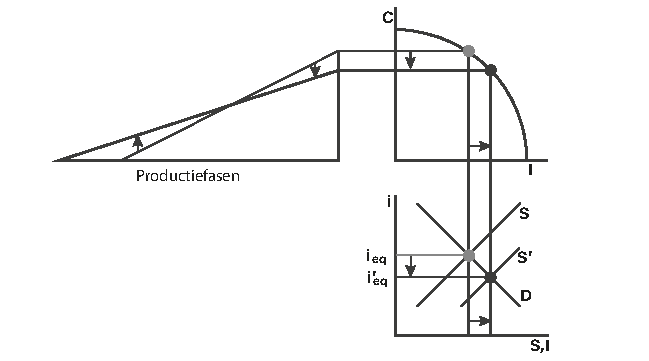
\includegraphics[width=\textwidth]{figures/fig32.pdf}
    \caption[Economische groei door investeringen en uitstel van consumptie\index{consumptie}]{Economische groei door investeringen en uitstel van consumptie\index{consumptie}}
    \label{fig32}
\end{figure}

Zuivere 100\% gedekte geldcertificaten veroorzaken geen toename in de geldhoeveelheid. Elk geldcertificaat dat als lening\index{lening} wordt uitgegeven, komt overeen met een vaste hoeveelheid van een marktgoed dat wordt aangehouden door de uitgever van het bewijs. Geld wordt als een echt marktgoed door de spaarders ter beschikking gesteld van de lener. Dat offer maakt economische middelen vrij die gebruikt kunnen worden in de vroege fasen van het productieproces\index{productieproces}, in plaats van voor consumptiegoederen\index{consumptiegoed}.

De dingen zien er heel anders uit wanneer fiduciaire middelen worden uitgegeven in plaats van geldcertificaten. Fiduciaire middelen worden uitgegeven zonder dat de bank\index{bank} geld in kas heeft. Niemand hoeft economische goederen op te offeren. Grafisch gezien stelt kredietexpansie via fiduciaire middelen leners in staat om pogingen te ondernemen om de productieketen te verlengen zonder de vereiste opoffering van consumptie\index{consumptie}. Ondernemers proberen met leningen een beweging boven de productiemogelijkhedencurve te maken met een omvang van investeringen en consumptie die de totale hoeveelheid beschikbare middelen overschrijdt. Op de kapitaalmarkt verschuift de aanbodcurve op een kunstmatige manier door de leenbare middelen te verhogen en daarmee de rentevoet te verlagen. De daling van de rente\index{rente} komt echter niet overeen met een toename van de spaartegoeden\index{spaartegoeden} waarmee de toegenomen investeringen zijn te financieren. Integendeel, lagere rentetarieven ontmoedigen het sparen juist.

De hoeveelheid geïnvesteerde middelen, I2 in het voorbeeld van Figuur 33, is veel groter dan de hoeveelheid gespaarde middelen, S2. De monetaire expansie\index{monetaire expansie} zorgt er niet alleen voor dat ondernemers denken dat ze meer middelen hebben dan ze in werkelijkheid bezitten, het zorgt er ook voor dat er minder middelen beschikbaar zijn door sparen te ontmoedigen en dus meer consumptie\index{consumptie} te stimuleren. Het verschil tussen I2 en S2 in deze grafiek is het kapitaal\index{kapitaal} dat ging naar de financiering van wat Mises zogenoemde \textbf{waninvesteringen} noemt -- investeringen die niet zouden zijn gedaan zonder verstoringen op de kapitaalmarkt, en waarvan de voltooiing niet mogelijk is zodra deze verstoringen aan het licht komen.\autocite{177} Het falen van de investering om de gewenste output te produceren leidt tot een krimp van de productiemogelijkhedencurve, aangezien de hoeveelheid beschikbare middelen afneemt. De productiedriehoek wordt korter en de productieketen krimpt.

\begin{figure}
\centering
    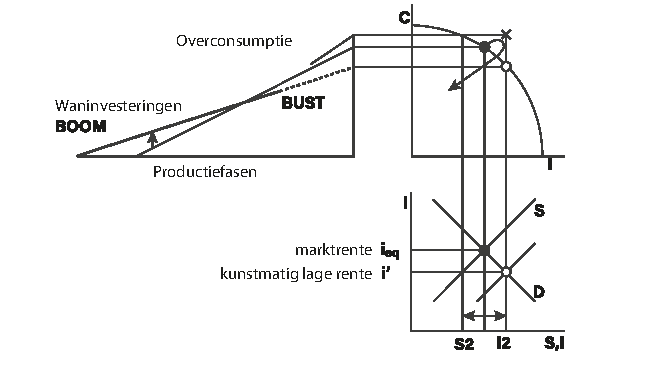
\includegraphics[width=\textwidth]{figures/fig33.pdf}
    \caption[Kredietexpansie met fiduciaire middelen en de conjunctuurcyclus\index{conjunctuurcyclus}]{Kredietexpansie met fiduciaire middelen en de conjunctuurcyclus\index{conjunctuurcyclus}}
    \label{fig33}
\end{figure}

De situatie is echter heel anders wanneer fiduciaire middelen worden uitgegeven in plaats van geldcertificaten, zoals geïllustreerd in Figuur 33. Fiduciaire middelen worden uitgegeven zonder dat de bank\index{bank} er de dekking voor bezit. Ze vereisen dus geen opoffering van economische goederen, door wie dan ook. Grafisch uit kredietexpansie door middel van fiduciaire middelen zich in het verlengen van de productieketen (de opwaartse pijl in de driehoek op Figuur 33) zonder de benodigde vermindering van de consumptie\index{consumptie} (de stippellijn in de driehoek en de witte stip in de PMC). Kredietnemende ondernemers proberen in feite om voorbij de productiemogelijkhedengrens te gaan met een hoeveelheid investeringen en consumptie\index{consumptie} die de totale hoeveelheid beschikbare middelen overschrijdt (het kruis in de PMC).

Op de kapitaalmarkt komen de opportuniteitskosten van kapitaal uit de opgeofferde consumptie en de opportuniteitskosten van consumptie zijn niet-gemaakte kapitaalinvesteringen. De rentevoet is de prijs die deze relatie regelt: naarmate mensen meer investeringen vragen, stijgt de rentevoet, waardoor meer spaarders worden gestimuleerd om meer van hun geld opzij te zetten om te sparen. Als de rente daalt, stimuleert dit producenten om meer te investeren in meer technologisch geavanceerde productiemethoden met een langere tijdsduur. Een lagere rente maakt dus langere productieketens met een hoge productiviteit mogelijk. Hierdoor kan de maatschappij evolueren van vissen met hengels naar vissen met grote door olie aangedreven boten.

Naarmate een economie zich ontwikkelt en steeds geavanceerder wordt, verandert het verband tussen fysiek kapitaal\index{kapitaal} en de markt voor uitleenbare middelen in werkelijkheid niet, maar het wordt wel ondoorzichtiger in de hoofden van mensen. Een moderne economie met een centrale bank\index{centrale bank} is gebaseerd op het negeren van deze fundamentele afweging en op de aanname dat banken investeringen kunnen financieren met nieuw gecreëerd geld zonder dat consumenten hoeven af te zien van consumptie\index{consumptie}. Het verband tussen het sparen en de uitleenbare middelen is dusdanig verbroken dat het niet eens meer in economische leerboeken wordt onderwezen. In een standaard leerboek wordt de aanbodcurve voor uitleenbaar geld afgebeeld als een rechte verticale lijn waarvan de grootte wordt bepaald door beleidsmakers. In het Keynesiaanse alternatieve universum bepalen centrale banken eenvoudigweg de geldhoeveelheid en de rentevoet en er wordt aangenomen dat de fysieke middelen vanzelf tevoorschijn zullen komen om de nominale monetaire fantasieën van de bank\index{bank} te realiseren.

Reële productiemiddelen kunnen natuurlijk niet in het leven worden geroepen door monetair beleid, dus het kunstmatig verlagen van de rente\index{rente} creëert onvermijdelijk een discrepantie tussen spaartegoeden\index{spaartegoeden} en uitleenbare middelen. Bij deze kunstmatig lage rente\index{rente} gaan bedrijven meer schulden aan om projecten te starten dan dat spaarders bereid zijn opzij te zetten voor de financiering ervan. Met andere woorden, de waarde van de uitgestelde consumptie\index{consumptie} is lager dan de waarde van het geleende kapitaal\index{kapitaal}. Zonder voldoende uitgestelde consumptie\index{consumptie} zullen er niet genoeg kapitaal\index{kapitaal}, land en arbeidskrachten worden overgeheveld van consumptiegoederen naar kapitaalgoederen van een hogere orde in de vroegste productiefasen. Er is immers geen spreekwoordelijke ``free lunch'' en als consumenten minder sparen, zal er minder kapitaal\index{kapitaal} beschikbaar zijn voor investeerders.

Dit tekort aan kapitaal\index{kapitaal} is niet direct zichtbaar omdat banken en de centrale bank\index{centrale bank} genoeg fiduciaire middelen kunnen uitgeven voor alle leners. Het creëren van nieuwe biljetten aan papiergeld of digitale tegoeden om het tekort aan spaargeld aan te vullen, vergroot niet op magische wijze de fysieke kapitaalvoorraad van de maatschappij. In plaats daarvan devalueert het de bestaande geldvoorraad en verstoort het de prijzen, waardoor producenten aan productieprocessen beginnen die meer kapitaal\index{kapitaal} vereisen dan er feitelijk beschikbaar is. Omdat steeds meer producenten zullen bieden op minder kapitaalgoederen\index{kapitaalgoederen} en middelen dan ze verwachten er te zijn, is het natuurlijke resultaat een stijging van de prijs\index{prijs} van de kapitaalgoederen\index{kapitaalgoederen} tijdens het productieproces\index{productieproces}. Dit is het moment waarop de manipulatie aan het licht komt, wat leidt tot de gelijktijdige ineenstorting van verschillende kapitaalinvesteringen die plotseling onrendabel worden tegen de nieuwe prijzen van de kapitaalgoederen\index{kapitaalgoederen}; de \emph{waninvesteringen}. De interventie van de centrale bank\index{centrale bank} in de kapitaalmarkt maakt het mogelijk dat er meer projecten worden ondernomen, maar vanwege de verstoring van de prijzen zullen investeerders verkeerde economische calculaties maken. Met andere woorden, interventie door de centrale bank\index{centrale bank} \emph{veroorzaakt} waninvesteringen. De interventie van de centrale bank\index{centrale bank} kan de hoeveelheid daadwerkelijk beschikbaar kapitaal\index{kapitaal} niet vergroten, dus de investeringsprojecten zullen uiteindelijk worden geconfronteerd met de harde economische realiteit, en moeten stop worden gezet. Het gevolg is dat het reële kapitaal\index{kapitaal} dat in de projecten is geïnvesteerd onnodig wordt verspild. Het stopzetten van deze projecten veroorzaakt tevens een stijging van de werkloosheid in de hele economie omdat een groot aantal mensen in veel sectoren hun onderneming zien mislukken of zich moeten aanpassen. Dit gelijktijdige economiebrede faillissement\index{faillissement} van bedrijven met overdreven investeringen wordt een \textbf{recessie\index{recessie}} genoemd.

Alleen met een goed inzicht in de werking van kapitaalstructuur en hoe rentemanipulatie de stimulans voor kapitaalaccumulatie vernietigt, kan men de oorzaken van recessies en de schommelingen van de conjunctuurcyclus\index{conjunctuurcyclus} begrijpen. De conjunctuurcyclus\index{conjunctuurcyclus} is het logische resultaat van de manipulatie van de rente\index{rente}, waardoor de kapitaalmarkt verstoort door de investeerders te laten denken dat ze meer kapitaal\index{kapitaal} kunnen verwerven dan beschikbaar is met het ondeugdelijke geld dat ze van de bank krijgen. In tegenstelling tot wat de Keynesiaanse animistische mythologie beweert, zijn conjunctuurcycli geen mystieke fenomenen die veroorzaakt worden door onvoorspelbare ``animal spirits''. Bij het maken van een herstelplan hebben centrale banken het het liefst dat de oorzaak van de cyclus buiten beschouwing wordt gelaten. Recessies zijn echter het onvermijdelijke logische gevolg van hun rentemanipulatie, net zoals tekorten het onvermijdelijke gevolg zijn van prijsplafonds. Keynesiaanse economie creëert de conjunctuurcyclus\index{conjunctuurcyclus} en verkoopt zichzelf vervolgens als de oplossing.

Een passende analogie om dit punt duidelijk te maken kan geleend (en verfraaid) worden uit het werk van Mises: stel je de kapitaalvoorraad van een samenleving voor als bouwstenen en de centrale bank\index{centrale bank} als een aannemer die ze gebruikt voor de bouw van huizen. Voor de bouw van elk huis zijn 10.000 bakstenen nodig en de projectontwikkelaar is op zoek naar een aannemer die 100 huizen kan bouwen, waar in totaal 1 miljoen bakstenen voor nodig zijn. Een Keynesiaanse aannemer die het contract graag wil binnenhalen, realiseert zich dat zijn kansen om het contract binnen te halen groter zijn als hij een offerte kan indienen waarin hij belooft 120 van die huizen te bouwen met maar 800.000 bakstenen. Dit is vergelijkbaar met rentemanipulatie: het vermindert het aanbod van kapitaal\index{kapitaal} terwijl de vraag ernaar toeneemt. In werkelijkheid zijn er voor 120 huizen 1,2 miljoen bakstenen nodig, maar er zijn er slechts 800.000 beschikbaar. De 800.000 bakstenen zijn voldoende om met de bouw van de 120 huizen te beginnen, maar niet om ze te voltooien. Als de bouw begint, is de ontwikkelaar erg blij dat hij 20\% meer huizen ziet voor 80\% van de kosten. De geweldige Keynesiaanse bouwkunde heeft ervoor gezorgd dat hij de 20\%, die hij nu bespaart, kan uitgeven aan een nieuwe zeilboot.

Helaas kan het bedrog niet blijven aanhouden, want uiteindelijk zal blijken dat de huizen niet kunnen worden afgebouwd en de bouw zal moeten worden stilgelegd. Niet alleen is de aannemer er niet in geslaagd om de 120 huizen op te leveren, maar hij zal zelfs helemaal geen huizen opleveren. In plaats daarvan heeft hij de ontwikkelaar achtergelaten met 120 onafgemaakte huizen, in feite nutteloze stapels bakstenen zonder dak. Het bedrog van de aannemer verminderde het kapitaal\index{kapitaal} dat door de ontwikkelaar werd uitgegeven en resulteerde in de bouw van minder huizen dan mogelijk zou zijn geweest met juiste prijssignalen. De ontwikkelaar zou 100 huizen hebben gehad als hij met een eerlijke aannemer in zee was gegaan. Door in zee te gaan met een Keynesiaanse aannemer die de cijfers manipuleert, blijft de ontwikkelaar zijn kapitaal\index{kapitaal} verspillen zolang het kapitaal\index{kapitaal} wordt toegewezen volgens een plan dat geen basis heeft in de realiteit. Als de projectontwikkelaar zich al in een vroeg stadium van de bouw van de 120 huizen bewust wordt van zijn fout, is het verspilde kapitaal\index{kapitaal} misschien heel beperkt en kan een nieuwe aannemer de overgebleven stenen gebruiken om 90 huizen te produceren. Als de ontwikkelaar onwetend blijft van de realiteit totdat het kapitaal\index{kapitaal} op is, zal hij eindigen met 120 onafgemaakte huizen die waardeloos zijn, omdat niemand zal betalen om in een huis zonder dak te wonen.

Wanneer de centrale bank\index{centrale bank} de rente\index{rente} tot onder de marktprijs manipuleert door banken meer geld te laten creëren door het verstrekken van leningen, verlagen ze tegelijkertijd de hoeveelheid spaargeld die beschikbaar is in de samenleving en verhogen ze de hoeveelheid die wordt gevraagd door leners. Dit terwijl ze ook het geleende kapitaal\index{kapitaal} sturen naar projecten die niet kunnen worden voltooid. Wanneer een overheid\index{overheid} het pad van het opblazen van de geldhoeveelheid is opgegaan, is er niet te ontkomen aan de negatieve gevolgen. Als de centrale bank\index{centrale bank} de monetaire expansie\index{monetaire expansie} stopt, stijgen de rentetarieven en volgt er een recessie\index{recessie} omdat veel van de gestarte projecten verlieslatend blijken te zijn en moeten worden opgegeven. Hierdoor komt de verkeerde allocatie van productiemiddelen en kapitaal\index{kapitaal} aan het licht. Als de centrale bank\index{centrale bank} haar inflatoire proces oneindig zou voortzetten, zou zij de omvang van de misallocaties in de economie alleen maar vergroten, waardoor nog meer kapitaal\index{kapitaal} wordt verspild en de onvermijdelijke recessie\index{recessie} nog pijnlijker wordt. Er is geen ontkomen aan het betalen van een flinke rekening voor de veronderstelde gratis lunch die Keynesiaanse gekken ons hebben opgedrongen.

Friedrich Hayek vergeleek kredietexpansie met het vangen van een tijger bij zijn staart. Als je de tijger eenmaal bij zijn staart hebt, begint hij te rennen en zijn er geen goede oplossingen meer.

\begin{blockquotebox}
We hebben nu een tijger bij de staart: hoelang kan deze inflatie\index{inflatie} nog doorgaan? Als de tijger wordt vrijgelaten zal hij ons opeten; maar als hij steeds sneller rent terwijl wij wanhopig blijven volhouden, zijn we nog steeds de pineut! Ik ben blij dat ik hier niet zal zijn om de uiteindelijke uitkomst te zien.\footnotemark
\end{blockquotebox}
\footautocite{178}


\section{Centrale planning van de kapitaalmarkt}

Fiduciaire middelen zijn financiële producten die op natuurlijke wijze zouden kunnen ontstaan op een vrije markt, maar het is volstrekt onwaarschijnlijk dat ze lang zouden overleven. Ze zouden op de markt kunnen ontstaan door de unieke aard van geld als een goed waarvan het enige doel is om het te ruilen voor iets anders, waardoor een claim op geld schijnbaar net zo goed is als geld door het feit dat ze beiden kunnen worden geruild voor goederen. Fiduciaire middelen zouden echter niet lang overleven op een vrije markt, omdat ze de uitgever ervan blootstelt aan het risico\index{risico} van faillissement\index{faillissement} als een bepaald percentage van hun schuldeisers probeert om de fiduciaire middelen weer in te wisselen voor geld.

Onder de goudstandaard\index{goudstandaard} werden fiduciaire middelen veel gebruikt, maar ze leidden tot periodieke financiële crises waarbij grote bedragen werden weggevaagd of sterk ontwaard. Fiduciaire middelen konden overleven onder een goudstandaard\index{goudstandaard} omdat een aanzienlijk deel van de totale geldhoeveelheid te allen tijde op de bank\index{bank} zou blijven staan. Veel eigenaren gaven er namelijk de voorkeur aan om hun geld op de bank\index{bank} te houden, waar het gebruikt kon worden voor het afwikkelen van betalingen tegen veel lagere kosten dan door het verplaatsen van fysiek goud\index{goud}. Persoonlijk betalen met fysiek goud\index{goud} buiten iemands woonplaats was praktisch onbetaalbaar, en de vooruitgang van transport- en telecommunicatietechnologie betekende dat steeds meer transacties van een individu plaatsvonden over lange afstanden. Dit resulteerde in een steeds groter percentage van het goud\index{goud} dat op de bank\index{bank} moest blijven staan om de verkoopbaarheid\index{verkoopbaarheid} ervan over afstand te vergroten. Elke keer dat een houder van een bankbiljet ervoor koos om het te verzilveren voor fysiek goud\index{goud}, koos hij voor een grote afname van de verkoopbaarheid\index{verkoopbaarheid} van zijn geld over afstand. Dit gaf banken een foutmarge bij de uitgifte van fiduciaire middelen, omdat ze wisten dat niet al hun klanten op hetzelfde moment om uitbetaling zouden vragen.

Deze veiligheidsmarge werkt zichzelf: hoe veiliger de bank\index{bank} is, hoe meer fiduciaire middelen ze uitgeeft, hoe minder veilig ze wordt en hoe vatbaarder ze zal zijn voor een bankrun. Deze bankruns zullen periodiek plaatsvinden en desastreus zijn voor veel betrokkenen. Een vrije markt in geld en bankieren zal waarschijnlijk banken en klanten die zich bezighouden met de uitgifte van ongedekt krediet\index{krediet} blijven wegvagen totdat het verschijnsel helemaal verdwijnt. De marginale kosten voor een bank\index{bank} om fiduciaire middelen te produceren zijn bijna nul, en een vrije bancaire markt zal fiduciaire middelen blijven leveren, totdat hun prijs\index{prijs} gelijk is aan de productiekosten. Dit betekent in feite dat de fiduciaire middelen zullen worden gedevalueerd totdat ze geldcertificaten worden en een nominale waarde hebben die gelijk is aan de dekking die er is om ze in te wisselen.

In de negentiende-eeuwse Verenigde Staten\index{Verenigde Staten} voorkwamen monopolistische bankvergunningen op concurrentie op de vrije markt de sanering van fiduciaire middelen.ervoor zorgde dat de fiduciaire middelen verdwenen. Zolang de toegang tot het bankwezen beperkt was, was het voor de gevestigde bedrijven winstgevend om fiduciaire middelen te produceren, ook al veroorzaakten ze periodieke crises en economische ineenstortingen. Periodieke overheidsinterventies in het banksysteem en de oprichting van de eerste en tweede centrale banken van de VS zouden de banken helpen beschermen tegen de gevolgen van ongedekte kredietexpansie op de vrije markt. Een grote financiële crisis in 1907 richtte de aandacht van de leiders van de financiële sector op de noodzaak om een derde monopolistische centrale bank\index{centrale bank} op te richten die klaarstond om bankinstellingen te redden in tijden van financiële crises. In 1913 werd de \textit{U.S. Federal Reserve Act\index{Federal Reserve Act}} aangenomen en kreeg de nieuwe centrale bank\index{centrale bank} het inherent tegenstrijdige tweeledige mandaat om de waarde van de valuta te beschermen en tegelijkertijd banken te redden van financiële crises. In de afgelopen eeuw bestond de prijs voor het beschermen van ongedekte kredieten tegen een juiste beoordeling door de markt, uit het constant ontwaarden van de munt. Terwijl in de negentiende eeuw de uitgifte van fiduciaire middelen financiële crises en onrust veroorzaakte, bleef dit relatief binnen de perken en beperkt tot mensen die vrijwillig betrokken waren bij deze financiële instellingen. De eigenaars van goud\index{goud} hadden niets te vrezen, aangezien de marktprijs van hun geld grotendeels onaangetast bleef. In de twintigste eeuw werden financiële crises bijna altijd verzacht en opgelost door de devaluatie van het geld dat in handen was van mensen die niet eens betrokken waren bij de insolvabele instituten.

In plaats van een manier te bieden om investeringen en productiviteit te verhogen, is kredietexpansie ongedekt door reële besparingen in de negentiende eeuw een recept gebleken voor financiële crises en de oorzaak van de vernietiging van gezond geld\index{gezond geld} in de twintigste eeuw. Om de financiële instellingen te beschermen tegen de gevolgen van ongedekte leningen, werd een socialistische centrale planningsinstantie ingesteld voor voor de markt voor geld en kapitaal\index{kapitaal} aangesteld de belangrijkste markt en het integrale onderdeel van alle andere markten\index{markten}.

Hoewel de meeste mensen denken dat socialistische samenlevingen tot het verleden behoren en dat marktsystemen heersen over kapitalistische economieën, kan een kapitalistisch systeem in werkelijkheid niet functioneren zonder een vrije kapitaalmarkt. De prijs\index{prijs} van kapitaal\index{kapitaal} dient te ontstaan door de interactie van vraag en aanbod en de beslissingen van kapitalisten horen te worden gestuurd door accurate prijssignalen. Recessies en financiële crises kunnen het best worden begrepen als het falen van kapitaalmarkten wanneer centrale planning de monetaire vrijheid beperkt. De bemoeienis met de kapitaalmarkt door monopolistische centrale banken is de oorzaak van recessies en financiële crises. Toch schrijft de meerderheid van politici, journalisten en academici deze centraal geplande rampen steevast toe aan het kapitalisme\index{kapitalisme}.

De mislukking die optreedt bij centrale planning op de kapitaalmarkt wordt de conjunctuurcyclus\index{conjunctuurcyclus} genoemd, zoals uitgelegd in de Oostenrijkse conjunctuurtheorie. Het is dus geen wonder dat dit disfunctioneren wordt behandeld als een normaal onderdeel van markteconomieën, want in de hoofden van moderne economen is een centrale bank\index{centrale bank} die de rente\index{rente} controleert immers een normaal onderdeel van een moderne markteconomie. Een centrale bank\index{centrale bank} is echter net zo\textquotesingle n normaal onderdeel van een kapitaalmarkt als een monopolistisch aardappelagentschap een normaal onderdeel is van aardappelmarkten.

Schrijvers van de Oostenrijkse School\index{Oostenrijkse School} hebben de monetaire geschiedenis nauwgezet gedocumenteerd in een aantal boeken die sterk zijn aan te raden, waarin de Oostenrijkse theorie wordt gebruikt om ons inzicht in de geschiedenis te verhelderen. Vaak wordt deze vertroebeld door de behoefte van overheidshistorici om de acties van de staat en zijn monetaire rampen te verbloemen. Vooral Hayek\textquotesingle s \emph{Monetary Nationalism and International Stability} , Rothbard\textquotesingle s \emph{America\textquotesingle s Great Depression} en \emph{A History of Money and Banking in the United States}, en Ferdinand Lips\textquotesingle{} \emph{Gold Wars} zijn goede voorbeelden. Deze geschiedenis wijst op een aantal ongelukkige, rampzalige en terugkerende patronen in de ontwikkeling van het moderne bankwezen en het overheidsbeleid.

Op de korte termijn hopen regeringen en centrale bankiers hun doelen te bereiken door geld te ontwaarden om kredietschepping en uitgaven voor belangrijke doelen te financieren. Regeringen denken misschien dat ze de economie stimuleren of mensen beschermen tegen de gevolgen van vrije markten\index{markten}, maar door het geld te devalueren om deze doelen te bereiken, creëren ze waninvesteringen en zaaien ze de kiem voor grote schade op de lange termijn. Pogingen om de economie te redden van de onvermijdelijke crises die daar het gevolg van zijn, resulteren in verdere kredietschepping en reddingsoperaties die onverantwoord gedrag aanmoedigen, de verkwisters belonen en de voorzichtige mensen straffen. Op die manier zorgen centrale banken er eigenlijk voor dat de conjunctuurcyclus\index{conjunctuurcyclus} een vast onderdeel wordt van een economie en dat hun macht over de markt groeit. Na verloop van tijd is het resultaat de vernietiging van kapitaal\index{kapitaal}, geld, het vermogen om te sparen en van de arbeidsdeling\index{arbeidsdeling} zelf. Geld in handen geven van een overheidsmonopolie is verre van een wondermiddel; het vernietigt de fundamenten waarop de menselijke samenleving en de moderne kapitalistische beschaving\index{beschaving} zijn gebouwd.
